\chapter{Intelligent History}
\label{ch:Intelligent-History}

To enable the investigation of our hypothesis, we developed Intelligent History,\footnote{\url{https://github.com/Alison-Li/intelligent-history}, verified 5/22/2022.} a prototype plugin for IntelliJ IDEA.
We describe the design and features of Intelligent History in \autoref{sec:Design} and elaborate on the implementation
for suggesting potentially more meaningful comments in \autoref{sec:Heuristics}.
In \autoref{sec:Predictions}, we discuss the use cases we envision Intelligent History to be able to effectively support.

%%%%%%%%%%%%%%%%%%%%%%%%%%%%%%%%%%%%%%%%%%%%%%%%%%%%%%%%%%%%%%%%%%%%%%
\section{Design}
\label{sec:Design}

As part of an effort to reduce the cognitive and temporal costs of software history exploration, we chose to develop a plugin to augment the existing rich features an \entity{IDE} already provides.
Unlike a stand-alone desktop or web application, a plugin minimizes the number of external application windows a developer needs to maintain and explore to gain context around revisions since the information Intelligent History offers would be integrated within the \entity{IDE}.
The IntelliJ \entity{IDE} provides a built-in Git client \entity{GUI} for navigating a software project's revision history and navigating revisions. 
In particular, the ``Show History'' feature in IntelliJ is available for directories and files, and displays a history of commits that have affected a single file or directory.
\autoref{fig:IntelliJ-Overview} shows IntelliJ with a file's commit history visible.
As a plugin, Intelligent History integrates with IntelliJ's ``Show History'' feature seamlessly as the plugin adds actions that can be invoked from a toolbar in IntelliJ's existing interface for exploring a file's commit history. 
This makes the features of Intelligent History complimentary to IntelliJ's existing version control interface.

We designed Intelligent History to support the following questions a developer might ask when searching for code rationale information in a file's revision history:

\begin{enumerate}
    \item ``Which commits are likely to be meaningful for understanding the decisions and choices involved in the evolution of this file?''
    \item ``Is there an interesting discussion or rationale that motivated the changes in a commit?''
\end{enumerate}

Intelligent History has the following features:

\begin{itemize}
    \item Commit highlighting to automatically detect and distinguish important commits from less important commits. The determination of less important commits is based on a set heuristics in the form regular expressions applied to the diff content of commits.
    \item A ``diff metadata'' summary, which shows the categorization of code changes detected in a commit according to the heuristics used for determining less important commits.
    \item Integrated Jira issue retrieval and presentation, along with metadata information about the Jira issue.
\end{itemize}

\begin{figure}
    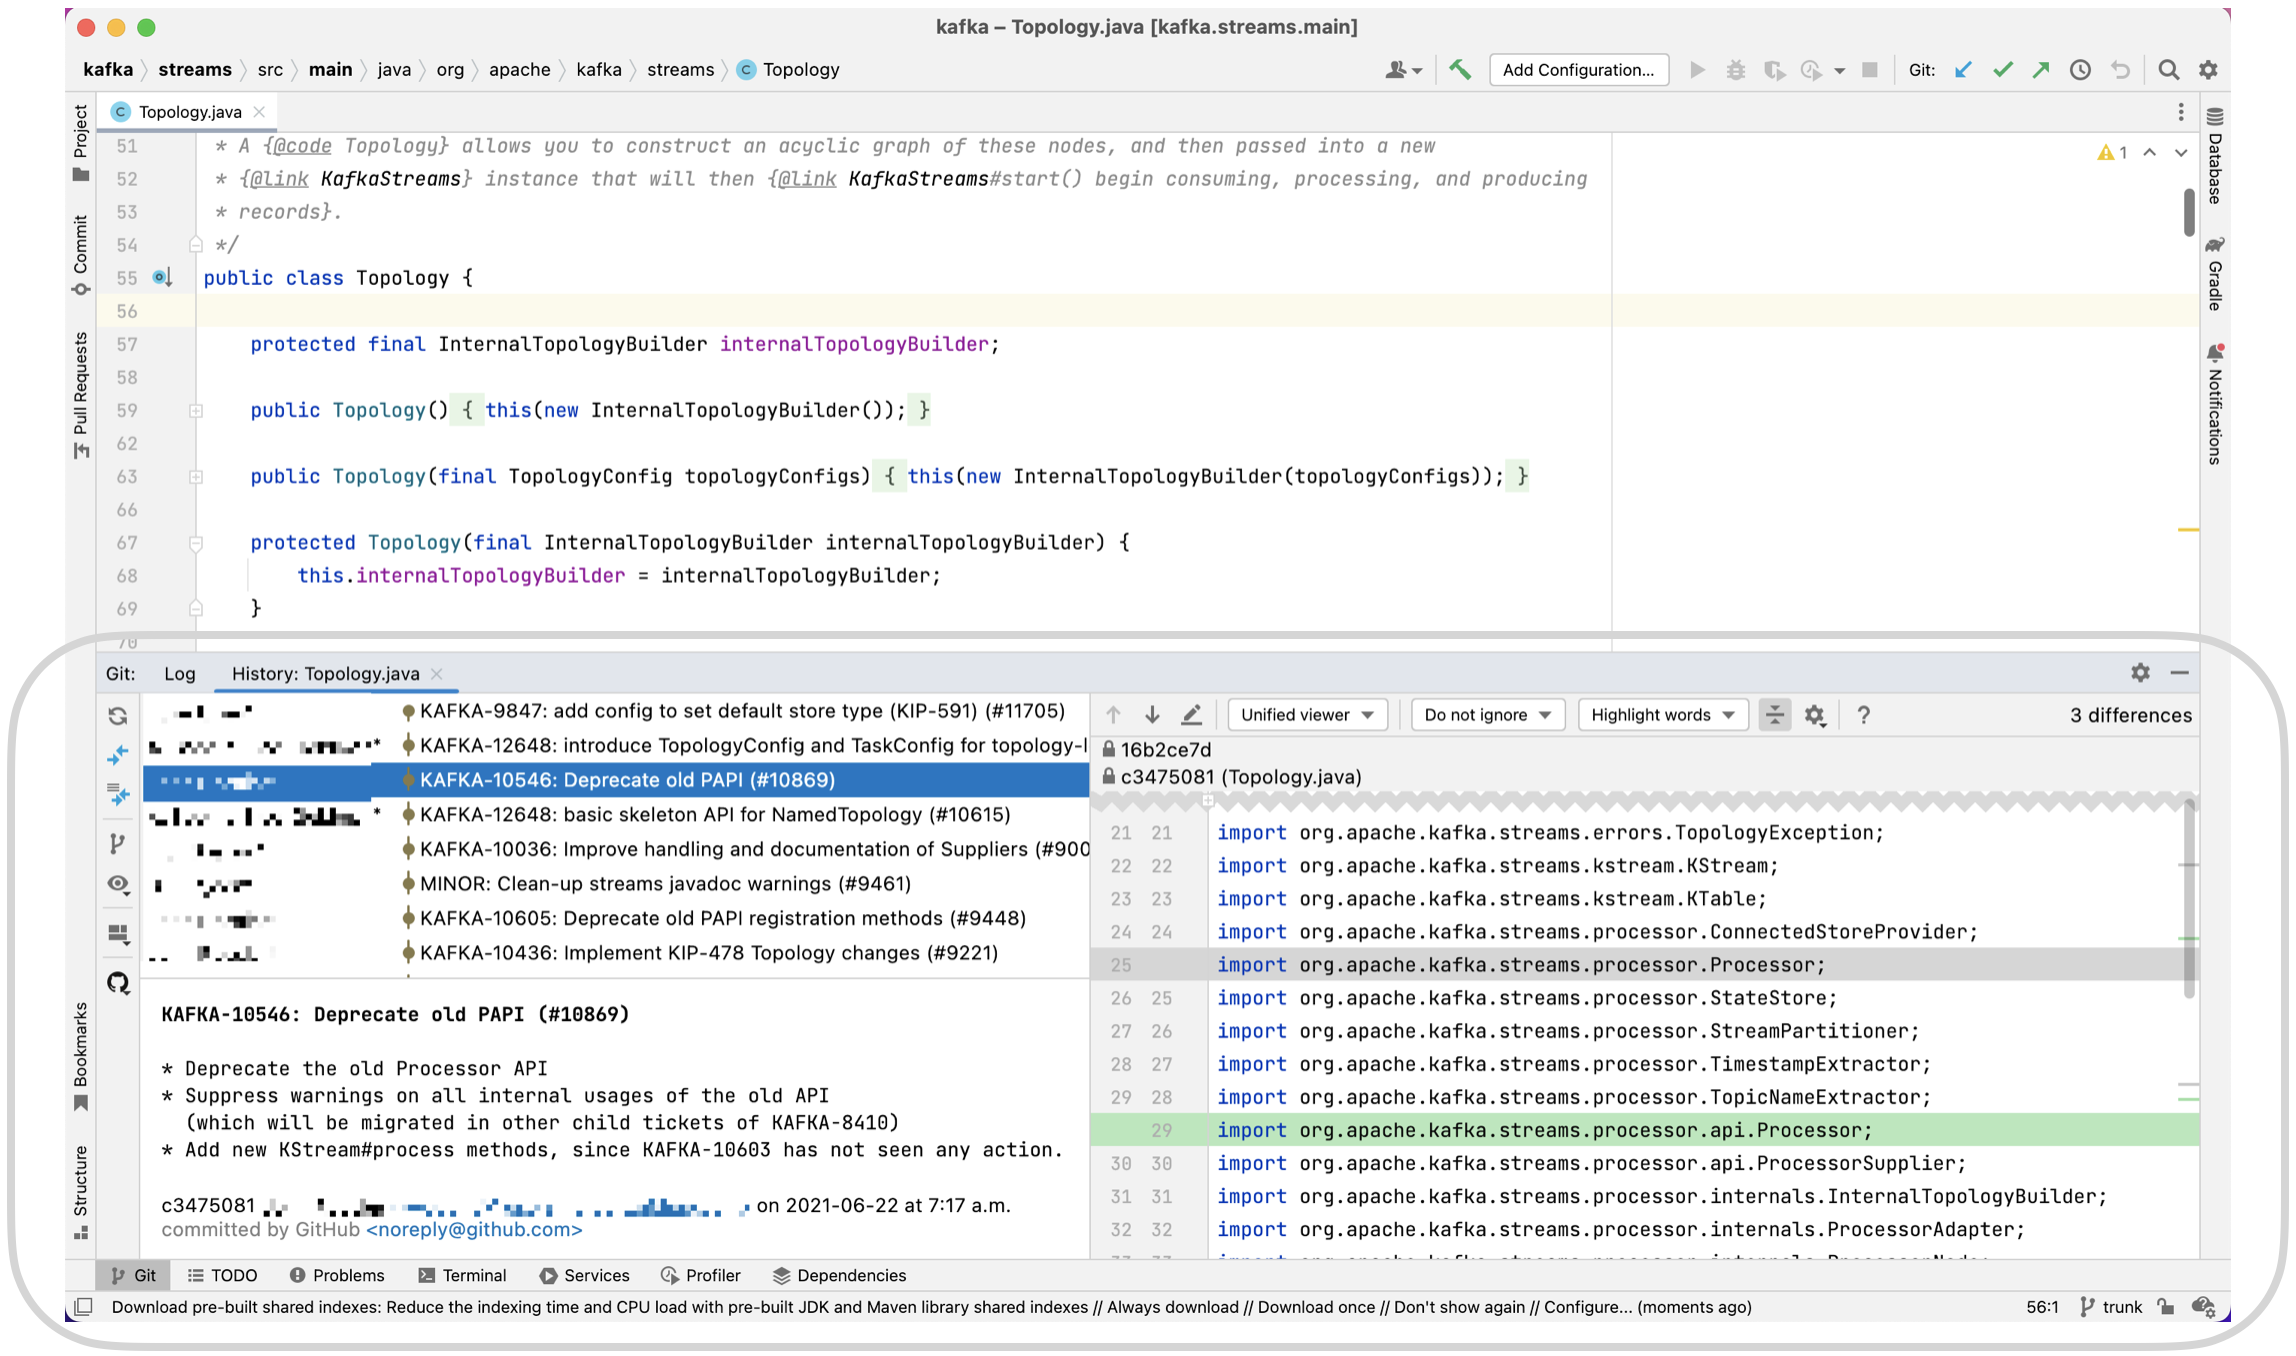
\includegraphics[width=\textwidth]{./images/intellij-overview.png}
    \caption{
        IntelliJ IDEA overview with the built-in Git client displayed on the bottom half. Shows the commit history for the \class{Topology} class in Apache Kafka.
    }
    \label{fig:IntelliJ-Overview}
\end{figure}

%%%%%%%%%%%%%%%%%%%%%%%%%%%%%%%%%%%%%%%%%%%%%%%%%%%%%%%%%%%%%%%%%%%%%%
\section{Heuristics}
\label{sec:Heuristics}

%%%%%%%%%%%%%%%%%%%%%%%%%%%%%%%%%%%%%%%%%%%%%%%%%%%%%%%%%%%%%%%%%%%%%%
\section{Predictions}
\label{sec:Predictions}

%%%%%%%%%%%%%%%%%%%%%%%%%%%%%%%%%%%%%%%%%%%%%%%%%%%%%%%%%%%%%%%%%%%%%%
\endinput

Any text after an \endinput is ignored.
You could put scraps here or things in progress.